\documentclass[a4paper,12pt]{article}
\usepackage[a4paper,top=3cm,bottom=2cm,left=3cm,right=3cm,marginparwidth=1.75cm]{geometry}
\usepackage[brazil]{babel}
\usepackage[T1]{fontenc}
\usepackage[utf8]{inputenc}
\usepackage{amsmath}
\usepackage{MnSymbol}
\usepackage{wasysym}
\usepackage{hyperref}
\usepackage{color}
\definecolor{Blue}{rgb}{0,0,0.9}
\definecolor{Red}{rgb}{0.9,0,0}
\usepackage{esvect}
\usepackage{graphicx}
\usepackage{float}
\usepackage{indentfirst}
\usepackage{caption}
\usepackage{blkarray}
\newcommand\Mark[1]{\textsuperscript#1}
\usepackage{pgfplots}
\usepackage{amsfonts}
\newtheorem{definicao}{Definição}[section]
\newtheorem{teorema}{Teorema}[section]
\title{Relatório de Laboratório 1}
\author{Guilherme Philippi}
\begin{document}
\maketitle
\tableofcontents

\section{Introdução}

Este relatório tem como objetivo apresentar soluções de exercícios envolvendo \textit{grafos}, que foi um tema estudado por diversos matemáticos proeminentes. Pode-se dizer que em 1736 é que a teoria teve início, com base no artigo publicado por Leonhard Euler, sobre as 7 pontes de Königsberg \cite{grafos1}. Existe uma íntima relação entre Grafos e algoritmos \cite{grafos0}. Podemos, por exemplo, representar um algoritmo por um grafo. Nos apegaremos a este conceito. Assim, segue a definição:

\begin{definicao}
	Um grafo $G$ é um par ordenado da forma $(V(G),E(G))$, composto por um conjunto de \textit{vértices} $V(G)$, de arestas $E(G)$ e uma \textit{função de incidência} $\psi_{g}$ que, por sua vez, associa a cada aresta de $V(G)$ um par não ordenado de vértices (nem sempre distintos) de $E(G)$. É dito que as arestas \textit{ligam} os vértices, bem como denomina-se também tais vértices como \textit{extremidades} desta aresta.
\end{definicao}

Utilizando esta definição, pode-se denominar outras características das estruturas de um grafo. Assim, por exemplo, estudamos: \textit{ordem, tamanho, incidência, adjacência, vizinhança, laço} e \textit{elo}. Assim, os separamos por tipos, como grafo: \textit{finito, nulo, simples, pseudografo, completo, conexo} e \textit{bipartido}. Dentre estas, frisamos algumas definições a seguir.

\subsection{Classificações}

\begin{definicao}
	Um grafo que não possui laços (arestas que possuem o mesmo vértice como extremidades),bem como não possui arestas paralelas (arestas cujas extremidades são os mesmo vértices) e onde quaisquer dois vértices são ligados por uma aresta é denominado \textit{grafo completo}.
\end{definicao}

\begin{definicao}
	\textit{Grafo conexo} é o nome dado para o tipo de grafo onde é possível estabelecer um caminho de qualquer vértice para qualquer outro vértice dele. Caso contrário, temos um \textit{grafo desconexo}.
\end{definicao}

\begin{definicao}
	Chamamos de \textit{grafo bipartido} o grafo onde pode-se particionar o conjunto de vértices em dois, de modo que cada aresta possua extremidades em ambos os conjuntos.
\end{definicao}

Em especial, também podemos discutir \textit{caminhos} (tanto eulerianos quanto hamiltonianos), \textit{cliques, ciclos, árvores, dígrafos} e, por fim, \textit{grafos ponderados}. Aqui, é importante destacar a definição de \textit{grafo ponderado}, pois podemos representar os esquemas de distâncias (muito utilizado em modelagem na engenharia) com base neles.

\begin{definicao}
	Chamamos de \textit{grafo ponderado} o grafo que possui valores numéricos atribuídos as suas arestas.
\end{definicao}

Após isto, partimos para o estudo de \textit{matrizes de incidência e adjacência}. 

\subsection{Grafos como matrizes}

Seguem algumas definições importantes.

\begin{definicao}
	As extremidades de uma aresta são denominadas \textit{incidentes} à aresta, bem como esta aresta é \textit{incidente} às \textit{extremidades}.
\end{definicao}

\begin{definicao}
	Vértices distintos e incidentes à uma mesma aresta são denominados \textit{adjacentes}. Nesse sentido, arestas que possuem um vértice em comum são \textit{adjacentes} também.
\end{definicao}

\begin{definicao}
	Dois vértices distintos e adjacentes são denominados \textit{vizinhos}. O conjuntos de vértices \textit{vizinhos} geralmente é denotado por $N_{G}(v)$.
\end{definicao}

Assim, a partir de matrizes, é possível definir outras maneiras de representar um grafo, donde
\\

\noindent\textbf{Matriz de Incidência: }Cada coluna representa os vértices incidentes a determinada aresta. Assim, cada linha representa as arestas incidentes a cada vértice. Contamos 1 para aresta incidente ao vértice (ou vice-versa) e 2 se tivermos um laço. Observe a matriz de incidência de $G_1$ à seguir:
\[
\begin{blockarray}{ccccccc}
f & g & h & i & j & k \\
\begin{block}{(cccccc)c}
1 & 0 & 0 & 0 & 0 & 1 & A \\
0 & 0 & 1 & 1 & 0 & 0 & B \\
0 & 0 & 0 & 0 & 0 & 0 & C \\
1 & 1 & 0 & 1 & 0 & 1 & D \\
0 & 1 & 1 & 0 & 2 & 0 & E \\
\end{block}
\end{blockarray}
\]

\noindent\textbf{Matriz de Adjacência: }É uma tabela onde observa-se somente a relação de adjacência entre vértices. Caso um vértice seja adjacente a outro, bota-se número 1. No caso de um laço, bota-se 2. Observe a matriz de adjacência de $G_1$:
\[
\begin{blockarray}{cccccc}
A & B & C & D & E\\
\begin{block}{(ccccc)c}
0 & 0 & 0 & 1 & 0 & A \\
0 & 0 & 0 & 1 & 1 & B \\
0 & 0 & 0 & 0 & 0 & C \\
1 & 1 & 0 & 0 & 1 & D \\
0 & 0 & 0 & 0 & 2 & E \\
\end{block}
\end{blockarray}
\]

Por último, temos alguns resultados sobre \textit{grau de um vértice}. Assim, seguem outras definições, com a prova de 2 resultados na sequência.

\begin{definicao}
	O \textit{grau} de um vértice é o número de arestas incidentes a ele. Cada laço conta como duas arestas. O vértice com \textit{grau} zero é chamado de \textit{vértice isolado}.
\end{definicao}
\begin{itemize}
	\item $d_{G}(v)$: É o grau do vértice $v$. Se $G$ é um grafo simples (sem laços ou arestas paralelas), então $d_{G}(v)$ denota o número de vizinhos de $v$ em $G$.
\end{itemize}

\begin{teorema}
	Para todo grafo $G(V(G),E(G))$, com $m$ arestas, vale:
	$$
	\sum\limits_{v\in V}{d_{G}(v)=2m}.
	$$
\end{teorema}
 Considere a matriz de incidência M do grafo G. Para saber o grau de um determinado vértice basta olharmos para sua linha correspondente e somarmos os valores contidos na linha. Note que somar os valores presentes em todas as linhas é o mesmo que somar os valores presentes nas colunas. Como temos $m$ colunas e cada aresta possui 2 vértices incidentes, segue que $\sum\limits_{v\in V}{d_{G}(v)=2m}$.

\begin{teorema}
	Em qualquer grafo, o número de vértices, cujo grau é ímpar, é par.
\end{teorema}
 Suponha que o número de vértices com grau ímpar seja ímpar. Note que a soma do grau de todos os vértices resulta em um número ímpar(resultado aritmético). Somando este resultado com o grau dos demais vértices, cujo grau é par, obtemos um número ímpar. Absurdo, pois $\sum\limits_{v\in V}{d(v)=2m}$. Portanto, o número de vértices, cujo grau é ímpar, é par.
 \\

Iremos apresentar alguns problemas-exemplos da utilização de grafos, implementando algorítimos bem conhecidos na literatura. Utilizou-se o software GRAFOS \cite{grafos} para modelar e simular as soluções propostas, assim como segue na próxima seção.

\section{Desenvolvimento}
\subsection{Distribuição de Sensores}
 Em uma casa que busca ser automatizada (vide Figura ~\ref{fig:sensores}), realizou-se uma proposta do cabeamento utilizando a menor quantidade possível de matéria prima (Cabos) levando em consideração que todas as tomadas de ar mostradas na planta (pontos em vermelho) deveriam ser visitadas. Considerou-se que todos os vértices do grafo que define o sistema podem ter ligações entre si de maneira linear.
 
\begin{figure}[H]
	\begin{center}
		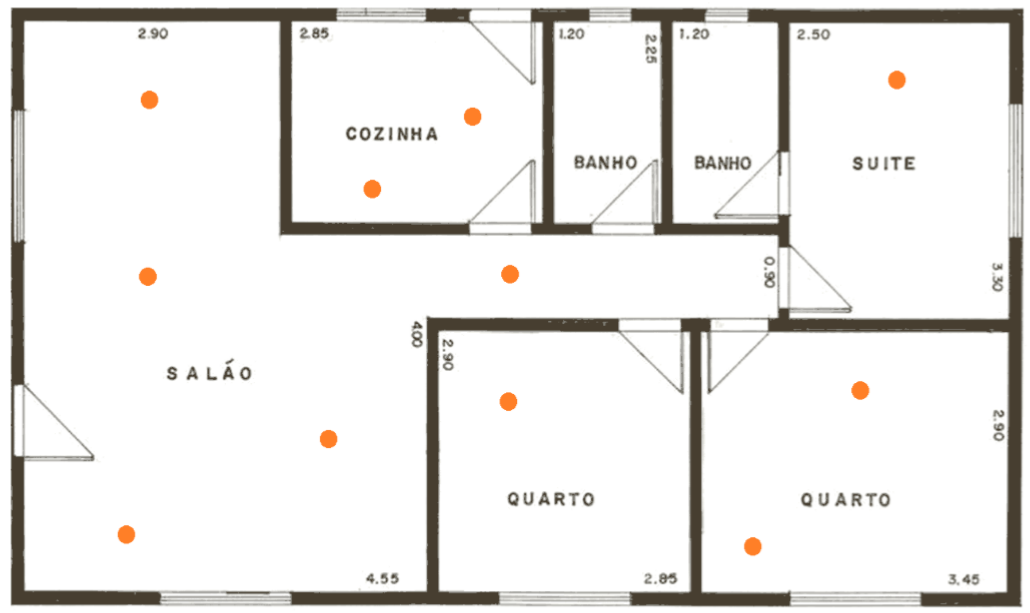
\includegraphics[width=0.8\linewidth]{sensores.png}
	\end{center}
	\caption{Distribuição dos sensores}
	\label{fig:sensores}
\end{figure}

Para solucionar este problema, com o auxilio do software GRAFOS, utilizou-se a Figura ~\ref{fig:sensores} como parâmetro, uma vez que a mesma está em perfeita escala, possibilitando-se que se calculasse as ponderações das arestas como as distâncias euclidianas dos pontos na imagem. Com isso, gerou-se o grafo completo mostrado na Figura ~\ref{fig:sensorescompleto}.

\begin{figure}[H]
	\begin{center}
		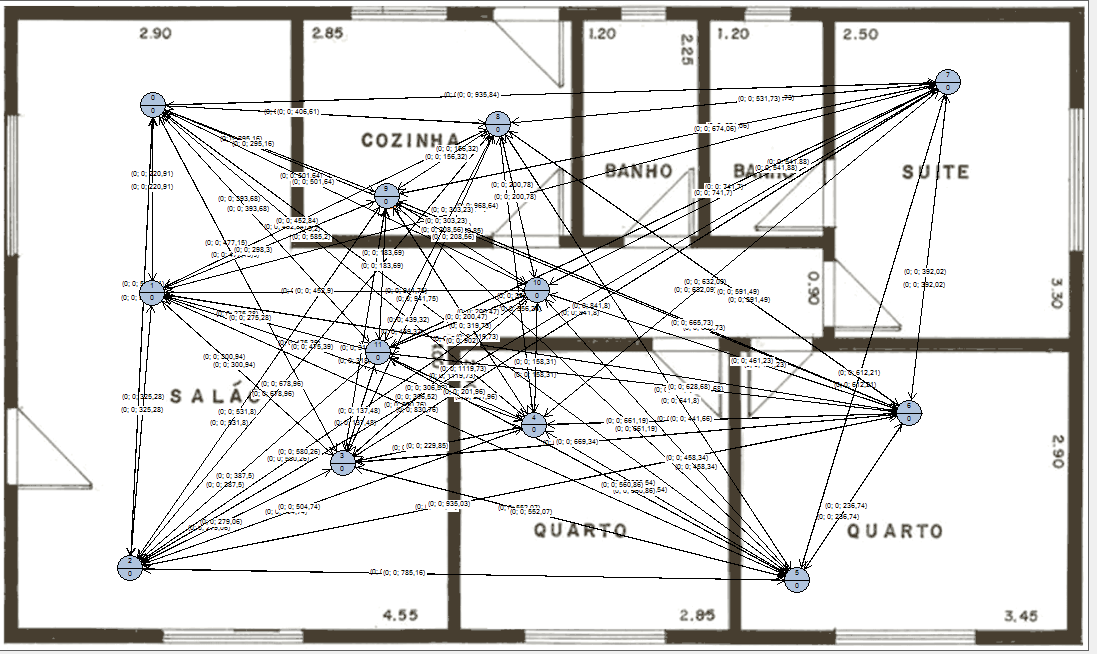
\includegraphics[width=0.8\linewidth]{sensorescompleto.png}
	\end{center}
	\caption{Grafo completo dos sensores}
	\label{fig:sensorescompleto}
\end{figure}

Com isso, pode-se utilizar o algorítimo de Kruskal, que busca uma árvore geradora mínima para um grafo conexo com pesos \cite{kruskal1990complexity}, ou seja, ele encontra um subconjunto das arestas que formam uma árvore incluindo todos os vértices onde o peso total desses, dado pela soma dos pesos das arestas da árvore, é mínimo. Observe o resultado obtido na Figura ~\ref{fig:sensoresconclusao}

\begin{figure}[H]
	\hspace{-1cm}
	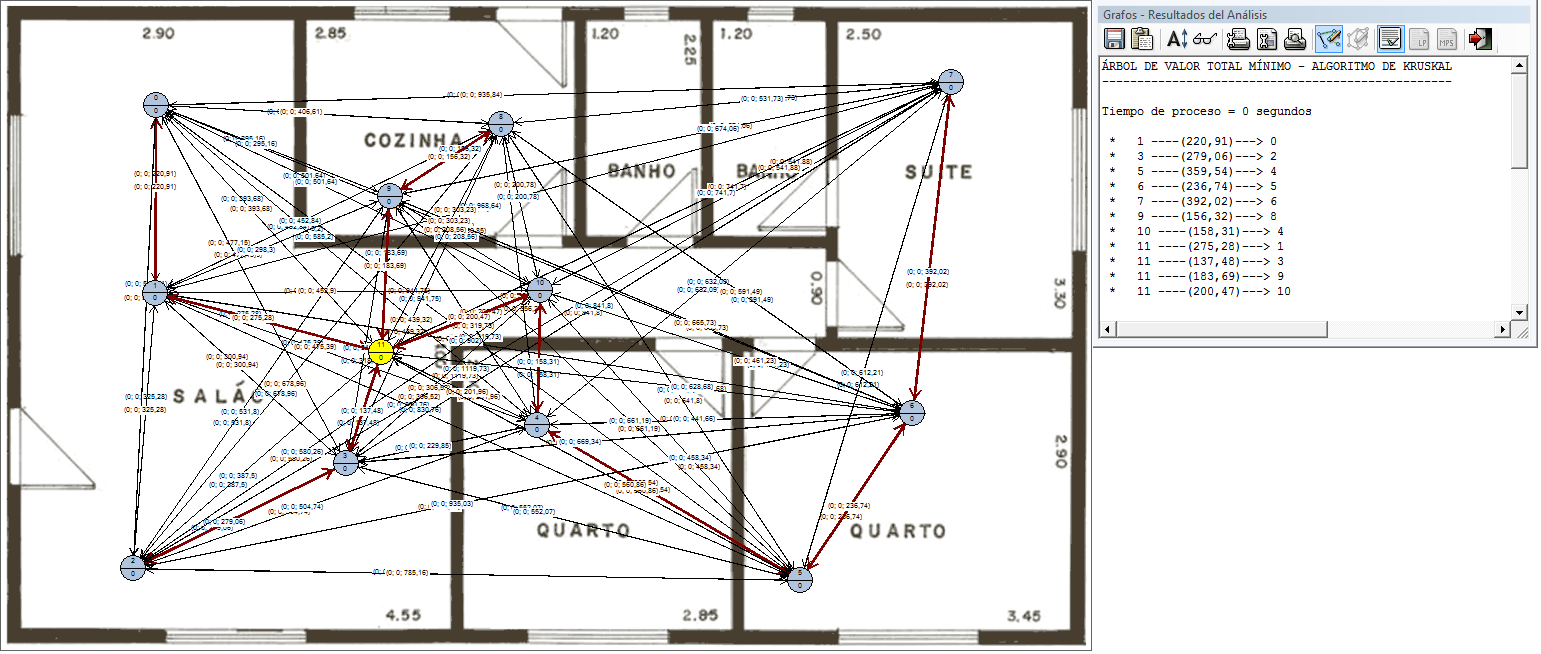
\includegraphics[width=1.2\linewidth]{sensoresconclusao.png}
	\caption{Aplicação do algorítimo de Kruskal no grafo completo}
	\label{fig:sensoresconclusao}
\end{figure}

\subsection{Sistema de Posicionamento Global}

Outro excelente problema-exemplo envolvendo grafos está em obter o menor caminho entre dois pontos obedecendo um sistema de rotas. Aqui teremos como objetivo construir um GPS primitivo que permita calcular as menores rotas entre o ponto $2$ e os demais pontos marcados no mapa da Figura ~\ref{fig:mapa}.

\begin{figure}[H]
	\begin{center}
		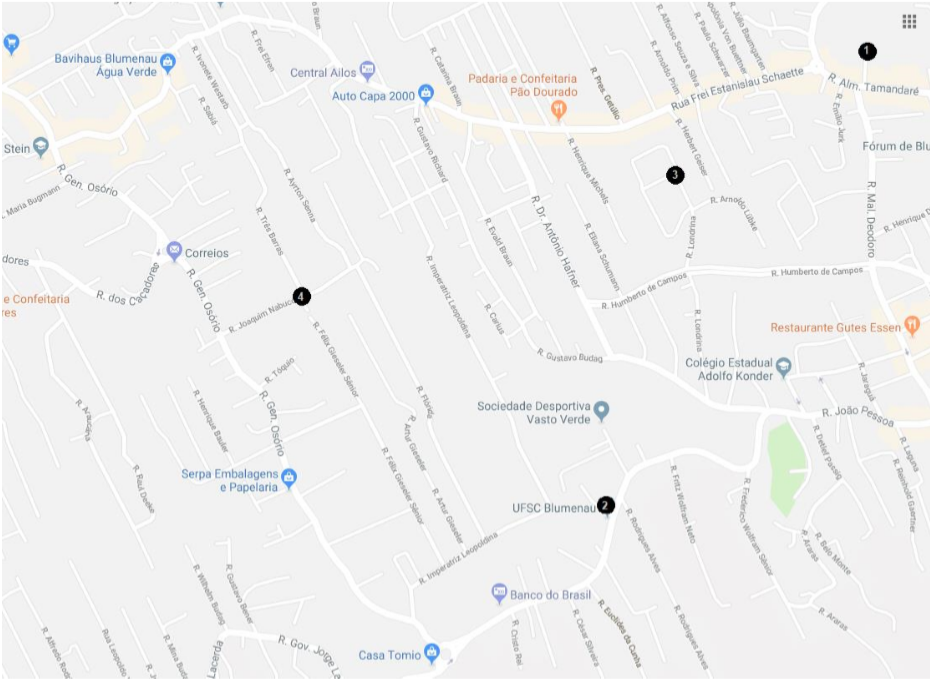
\includegraphics[width=0.85\linewidth]{mapa.png}
	\end{center}
	\caption{Mapa de rotas possíveis entre os pontos}
	\label{fig:mapa}
\end{figure}

\subsubsection*{Caminho do ponto 2 até 1}

Semelhante a Figura ~\ref{fig:sensores}, o mapa ilustrado na Figura ~\ref{fig:mapa} também está em perfeita escala, nos permitindo utilizá-lo como parâmetro para o software GRAFOS. Assim foi feito, obtendo os possíveis caminhos representados pelo grafo ponderado da Figura ~\ref{fig:mapa1} (note que somente os caminhos validos estão presentes, ou seja, não fora levado em consideração os caminhos demasiadamente longos).

\begin{figure}[H]
	\begin{center}
		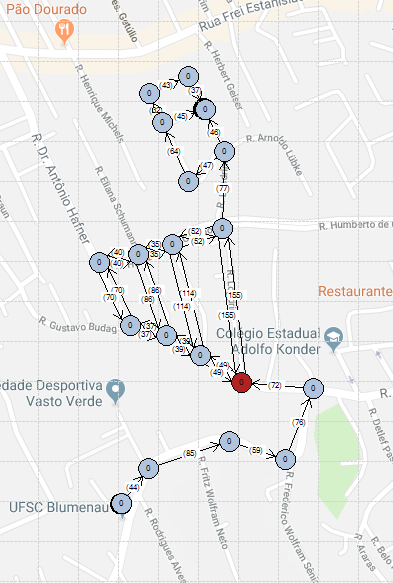
\includegraphics[width=0.45\linewidth]{cam1.png}
	\end{center}
	\caption{Mapa de rotas possíveis entre os pontos 2 e 1}
	\label{fig:mapa1}
\end{figure}

Com este grafo montado, podemos utilizar o algorítimo de Dijkstra, concebido pelo cientista da computação holandês Edsger Dijkstra em 1956 e publicado em 1959 \cite{dijkstra1959note}, que soluciona o problema do caminho mais curto num grafo dirigido (ou não) com arestas ponderadas não negativas, em tempo computacional $O(m + n \log{n})$ onde m é o número de arestas e n é o número de vértices. Assim sendo, obtivemos o caminho representado pela Figura ~\ref{fig:mapa1sol}

\begin{figure}[H]
	\begin{center}
		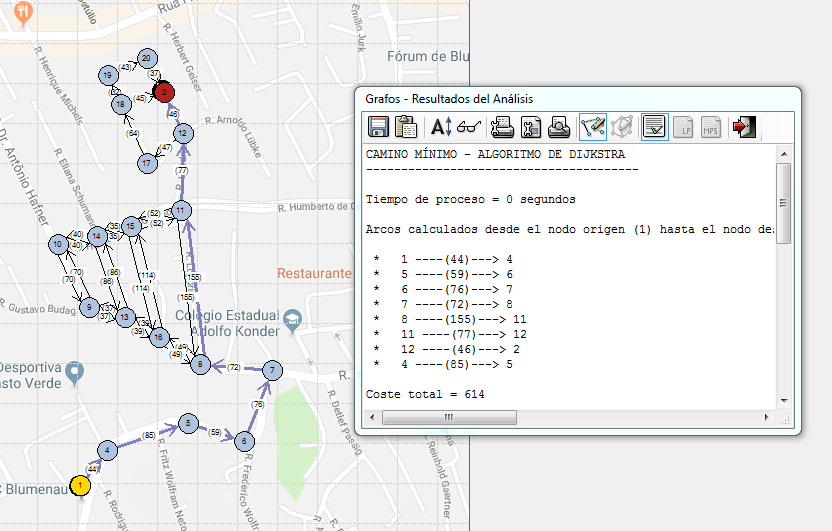
\includegraphics[width=0.7\linewidth]{cam1sol.png}
	\end{center}
	\caption{Mapa de rota mais curta entre os pontos 2 e 1}
	\label{fig:mapa1sol}
\end{figure}

\subsubsection*{Caminho do ponto 2 até 3}
Da mesma forma do destino anterior, construiu-se o grafo que melhor representa as possíveis rotas que ligam os pontos 2 e 3, como pode-se ver na Figura ~\ref{fig:mapa2}.

\begin{figure}[H]
	\begin{center}
		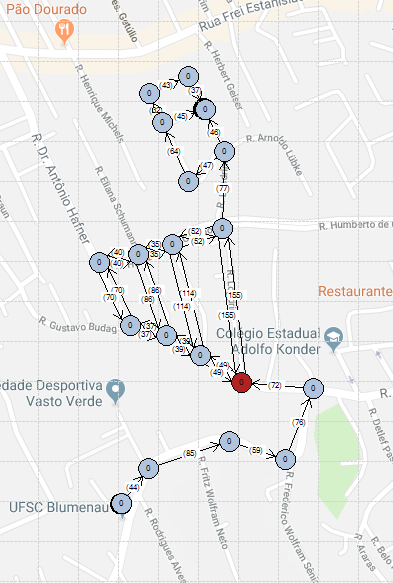
\includegraphics[width=0.45\linewidth]{cam2.png}
	\end{center}
	\caption{Mapa de rotas possíveis entre os pontos 2 e 3}
	\label{fig:mapa2}
\end{figure}

Segue, na Figura ~\ref{fig:mapa2sol}, a representação do caminho mais curto obtido através da aplicação do algorítimo de Dijkstra.

\begin{figure}[H]
	\begin{center}
		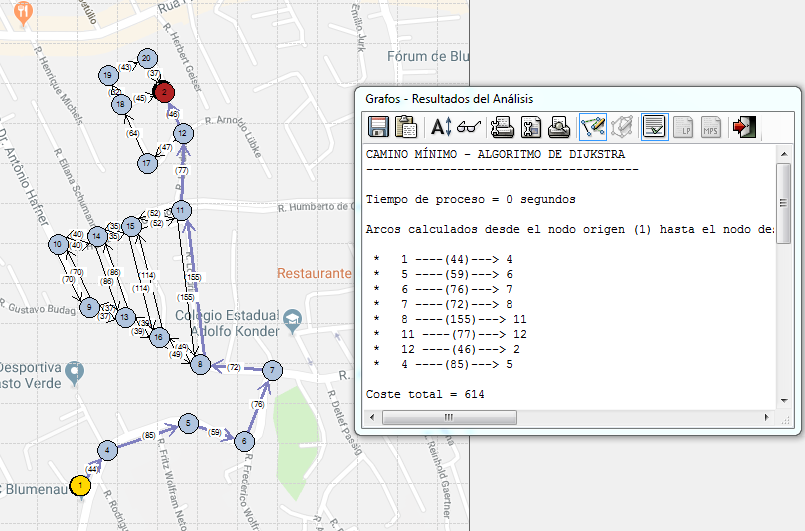
\includegraphics[width=0.8\linewidth]{cam2sol.png}
	\end{center}
	\caption{Mapa de rota mais curta entre os pontos 2 e 3}
	\label{fig:mapa2sol}
\end{figure}

\subsubsection*{Caminho do ponto 2 até 4}
Igualmente como os caminhos anteriores, construiu-se o grafo que melhor representa as possíveis rotas que ligam os pontos 2 e 4, como pode-se comprovar na Figura ~\ref{fig:mapa3}.

\begin{figure}[H]
	\begin{center}
		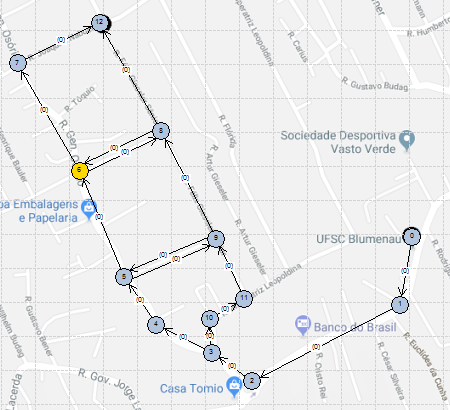
\includegraphics[width=0.6\linewidth]{cam3.png}
	\end{center}
	\caption{Mapa de rotas possíveis entre os pontos 2 e 4}
	\label{fig:mapa3}
\end{figure}

Segue, na Figura ~\ref{fig:mapa3sol}, a representação do caminho mais curto obtido através da aplicação do algorítimo de Dijkstra entre os pontos 2 e 4.

\begin{figure}[H]
	\begin{center}
		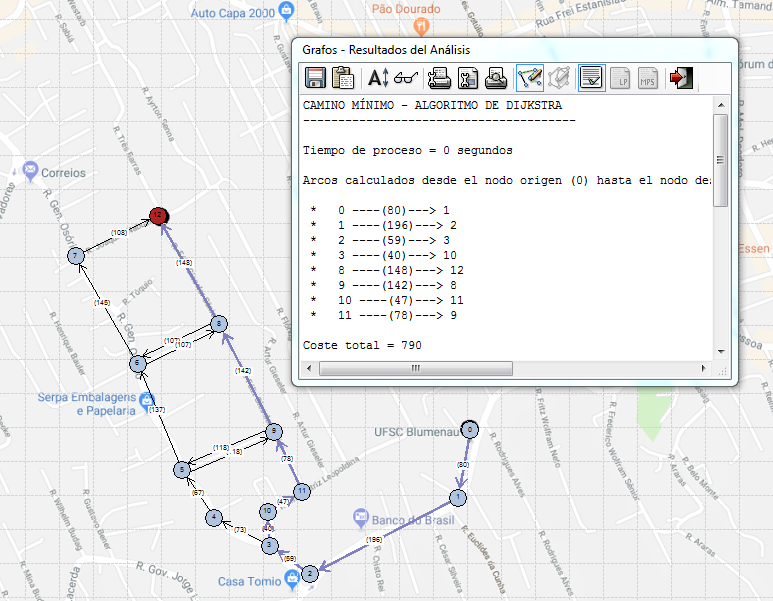
\includegraphics[width=0.8\linewidth]{cam3sol.png}
	\end{center}
	\caption{Mapa de rota mais curta entre os pontos 2 e 4}
	\label{fig:mapa3sol}
\end{figure}

\section{Considerações Finais}
Perceba que no problema-exemplo de posicionamento global alguns caminhos foram propositalmente omitidos, por serem considerados desprezáveis (trivialmente longos), donde que um resultado mais robusto contaria com a presença de um grafo completo, envolvendo todos os possíveis caminhos. Ressalta-se também que um estudo sobre a complexidade computacional dos algorítimos apresentados seria proveitoso para algum possível trabalho futuro.

Espera-se ter deixado claro para o leitor quais os princípios básicos envolvendo grafos, principais resultados e esboçado possíveis aplicações com o desenvolvimento proposto. Vale a ressalva de que a bibliografia contém uma grande quantidade de algorítimos diferentes envolvendo grafos e uma diversa gama de aplicações. 

Pede-se uma pequena pausa para a licença poética: Acreditamos que uma das mais belas características da representação dos grafos é que o conjunto de vértices $V$ aceita qualquer elemento, ou seja, pode ser tanto um sensor, quanto uma esquina. Daí vem o grande poder de abstração da representação de grafos.

\phantomsection
\addcontentsline{toc}{section}{Referências}

\bibliographystyle{unsrt}
\bibliography{references}

\end{document}
